In essence, \emph{margin trading} denotes the act of \emph{trading with
borrowed funds instead of your own}. To prevent misuse, institutes that offer
margin trading require enough \emph{collateral} for these loans to be put aside 
such that debts to lenders can be settled in any case.

\subsection{Terminology}

In this paper we distinguish between 
\begin{description}
 \item[long positions] that hold an actual asset,
 \item[borrowed positions] that received a market pegged asset (e.g. bitUSD)
                           for a collateral and
 \item[short positions] that sold the borrowed asset at the market leaving the
                        trader only with the locked collateral. 
\end{description}

A margin call is when your collateral is sold to the market automatically to
prevent further loss and ensure you do not default on your loans. Margin calls
are executed using one or more market orders; as such, order book liquidity at
the time of these orders will affect the extent of the losses you incur from
the liquidation. 

\subsection{Price Feed/Settlement Price}

The price feed is the external price of an asset (relative to BTS) fed into the
network by the witnesses~\cite{bts:financial}. The price is derived from the
median of the proposed price of all witnesses to prevent manipulation by
dishonest witnesses. This price furthermore, serves as the price for
settlement requests of long positions (see below).

\subsection{Collateral}

The collateral ratio can be derived by
\begin{align*}
 \text{ratio} = \frac{\text{debt}}{\text{collateral}} \;/\; \SP\;.
\end{align*}

Any additional collateral above the maintenance collateral is only required to
protect the position against margin calls due to volatility.

\subsection{Debt, Collateral and Swan}

In the case of market pegged assets, such as bitUSD, bitEUR, bitCNY, etc.,
where the BitShares network issues new shares~\cite{bts:financial}, it has to
be ensured that the collateral is always sufficient to cover the debts. Since
all SmartCoins are issued by the BitShares network, the overall debt equals the
supply of that particular asset.

In liquid markets, an equilibrium between collateral and debt is reached at the
price
\begin{align}
 \text{debt} &= \text{collateral} \cdot \text{price}
\end{align}
This price is called Black Swan Price (\SWAN) and indicates the price at which
all collateral could pay off all debt.
\begin{align}
 \Rightarrow\quad\text{\SWAN\ price} &= \text{debt} / \text{collateral}
\end{align}

\subsection{Margin Calls}

However, since markets do not have all their liquidity at the spot price we
need a back-off and start closing borrow positions earlier to prevent a black
swan event. In BitShares, the back-off factor is called \emph{Maintenance
Collateral Ratio (\MCR)} and derives the position-specific Margin Call Price
(\MCP) by:
\begin{align}
 \MCP = \frac{\text{dept}}{\text{collateral}} \cdot \MCR
\end{align}
The \MCR\ is a asset-specific parameter defined by the witnesses which can
change at any time.  It is derived from the median of the proposed \MCR s of
all active witnesses such that only the majority of witnesses can manipulate
this parameter. A commonly agreed value for the \MCR\ is \num{1.75} or 175\%.

Note that, once you have borrowed an asset from the BitShares network, your
position and exposure does not change (assuming you are not margin called). The
reason for this is very simple: You still hold all the borrowed asset in your
account that is required to pay of contract and release your collateral again.

%%%%%%%%%%%%%%%%%%%%%%%%%%%%%%%%%%%%%%%%%%%%%%%%%%%%%%%%%%%%%%%%%%%%%%%%%%%
Example:
When you borrow \SI{100}{USD} from the network and put \SI{50000}{BTS} as
collateral, your \MCP\ (assuming a \MCR\ of 175\%) would then derive to:
\begin{align*}
 \MCP = \frac{\SI{100}{USD}}{\SI{50000}{BTS}}\,\cdot\, 1.75 = \SI{0.0035}{USD\per BTS}
\end{align*}
Your collateral ratio depends on the price feed and derives to
\begin{align*}
 \text{ratio} = \frac{\SI{100}{USD}}{\SI{50000}{BTS}} \;/\; \SP\;.
\end{align*}
%%%%%%%%%%%%%%%%%%%%%%%%%%%%%%%%%%%%%%%%%%%%%%%%%%%%%%%%%%%%%%%%%%%%%%%%%%%

\subsubsection{Short Squeeze Protection}

A new feature in BitShares 2.0 is the protection of short/borrow positions
against short squeezes (rapidly falling price of BTS). A short squeeze implies
that short sellers are being squeezed out of their short positions (usually at
a loss). 

To protect shorts against short squeezes \textbf{in markets with low
liquidity}, margin calls only execute if the position's call price (\MCP) is
\textbf{above} the short squeeze protection price (\SQP).

The \SQP is derived by
\begin{align}
 \SQP = \frac{\SP}{\MSQR}
\end{align}

This behavior is motivated to ensure that short positions do not require to buy
on the ask-side even though there are bid orders above their own margin call
price.

%%%%%%%%%%%%%%%%%%%%%%%%%%%%%%%%%%%%%%%%%%%%%%%%%%%%%%%%%%%%%%%%%%%%%%%%%%%
Example:
Currently (November 2015), the \MSQR\ for the USD tracking asset in BitShares
has a value of \num{1.1} (e.g. 110\%). Assuming a feed price of $\SP =
\SI{0.005}{USD\per BTS}$ results in an \SQP\ or \SI{0.0045455}{USD\per BTS}.
Hence, the call price has to be higher than the \SQP\ and there must not be a
bid above your \MCP\ for a margin call to occur.
%%%%%%%%%%%%%%%%%%%%%%%%%%%%%%%%%%%%%%%%%%%%%%%%%%%%%%%%%%%%%%%%%%%%%%%%%%%

We summarize the margin call rules as follows:
\begin{center}
\noindent\framebox[.8\linewidth]{\parbox{.75\linewidth}{
          A \textbf{margin call} will occur any time the highest bid is
          \textbf{less} than the call price and \textbf{greater} than the Short
          Squeeze Protection Price, i.e.
          \begin{align}
           \text{highest bid}\; &< \;\MCP \\
           &\land\notag\\
           \text{highest bid}\; &> \;\SQP
          \end{align}}}
\end{center}

\subsubsection{Illustrative Description}

In order to simplify illustration we summarize the terms that have been
discussed in the previous paragraphs as follows:
\begin{description}
 \item[(Black) Swan Price:] The price at which the collateral equals the debt
 \item[Maintenance Collateral Ratio (\MCR)]: a ratio to define the margin call
       price as a function of the swan price.
 \item[Margin Call Price (\MCP):] Margin positions with a call price below this price
       may be margin called (see below).
 \item[Settlement Price (\SP):] The price at which a long position can request
       settlement against the least collateralized borrow position.
 \item[Maximum Short Squeeze Ratio (\MSQR):] This ratio defines the price to
       which shorts are protected against short squeezes.
 \item[Short Squeeze Protection Price (\SQP):] As long as the highest bid order
       is above this price, no margin calls will be executed. The \SQP\ defines
       the most that a margin position will ever be forced to pay to cover.
\end{description}

To illustrate the relation of prices and the impact of collateral, we have
depicted the prices in the following figure.

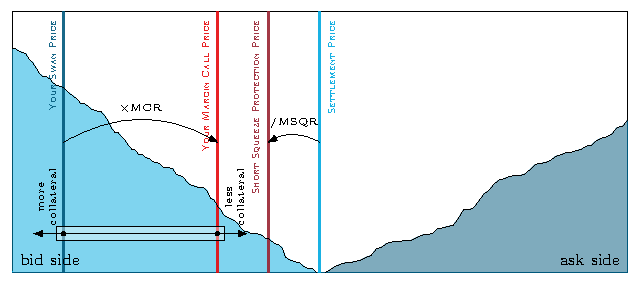
\includegraphics[width=.9\linewidth,page=1]{figures/dex-engine-def.pdf}

We see that the trader's swan price can be adapted by increasing (or
decreasing) the amount of collateral. Obviously, this has a direct consequence
on the position's margin call price because it is derived from the
asset-specific \MCR (e.g. 175\%).

We also see that the short squeeze protection price (\SQP) is derived from the
settlement price and the maximum short squeeze ratio (\MSQR) (e.g. 110\%).

\bigskip

When the price of BTS against an asset (e.g. USD) falls, the market moves
closer to a black swan event. To prevent a black swan, the BitShares
automatically performs margin calls.

The following figure shows the market (and the price feed) at a lower price. We
see that the position's \MCP\ is still below (here: left of) the short \SQP.
Hence, that particular position is not called yet. However, the risk being
margin called rises.

\includegraphics[width=.9\linewidth,page=2]{figures/dex-engine-def.pdf}

At this point it is strongly advised that traders check their markets and open
positions regularly, mitigating the risk of being margin called by reducing the
debt of your positions or increasing the collateral ratio with additional
collateral.

If the price falls further (as depicted in the next figure), the \SQP\ may
cross the \MCP and your position is in danger of being called. In this
particular example, however, there are still bid orders above your \MCP, which
results in no margin call, as of yet.

\includegraphics[width=.9\linewidth,page=3]{figures/dex-engine-def.pdf}

If, however, the all the bids above your \MCP\ disappear (either by being closed
or filled), you position will be force liquidated. 

\includegraphics[width=.9\linewidth,page=4]{figures/dex-engine-def.pdf}

This means, that all of the collateral will be used to buy just enough of the
borrowed asset (e.g. USD) to close the position. The remaining collateral will
be transfered back to the original position's owner.

\subsection{Settlement}

Any long position (i.e. holder of SmartCoins) can request a settlement to
convert their long position into the core asset BTS. The settlement has a
asset-specific delay of 24h and settles at the settlement price which is
identical to the feed price. By this it is ensured that 1 bitUSD is always
worth at least \$1 worth of BTS.

\subsection{Discussion}

A margin position will be forced to sell its collateral anytime the highest
offer to buy the collateral is less than the call price (USD/BTS).

The market defines everything (as it should).
The market sets the value of BTS in terms of BitUSD based on the highest offer
to buy BTS with BitUSD.
Once we know the market value, we can trigger margin calls.

There is ONE edge case and that is for thin markets.  In this edge case the
market cannot define the value of BTS in terms of BitUSD.  This is where we use
the SQP as the lower bound on the value of BTS in terms of BitUSD.
%%%%%%%%%%%%%%%%%%%%%%%%%%%%%%%%%%%%%%%%%%%%%%%%%%%%%%%%%
I get that it is illogical for a bid to stay
high, when he can lower his bid and force a margin call.  In a thin market this
is easy. A thick market would be more difficult. 

Its not logical to lower your bid when there are other bids still above the
margin call price; You may never get filled. All participants would need to
play the same game, or you would have to sell into the bid till the margin call
triggered, but this has a cost that may be more than the reward.

In addition, a short can always, at any time, manually close his position at
"cheap" (when bid is higher than his Margin Call Price), instead of waiting for
a forced liquidation at "expensive" (when bid falls below his Margin Call
Price).   

I guess they make sense in protecting the system from there
not being enough bid to cover a margin called short. Its only partial
protection though. I'm not sure its worth the distortion it creates.
Essentially incentivizing the bid to stay just above the SQP rate.

What are you suggesting should be changed, to make this wheel round?  Should
the short be called only when the feed drops below his margin call price
filling all available bids down to the SQP rate(10\%)?

I think so long as the markets determining the feeds are external to the Dex
and greater in volume the old rule is more practical, but with greater systemic
risk. Once the internal markets are leading the feed, I think this issue goes
away and really may be unnecessary.
%%%%%%%%%%%%%%%%%%%%%%%%%%%%%%%%%%%%%%%%%%%%%%%%%%%%%%%%%
\subsubsection{Liquid Markets}
\subsubsection{Thin Markets}
\subsubsection{Manipulative Bid-Orders}
